\chapter{Das LHCb-Experiment}  \label{kap:experiment}
Der Large Hadron Collider (LHC) an der internationalen Forschungseinrichtung CERN in Genf ist der derzeit größte Ringbeschleuniger der Erde. Er hat einen Durchmesser von ca. $27\kilo\meter$. Im Ring werden zwei geladene Teilchenstrahlen in gegenläufiger Richtung auf nahezu Lichtgeschwindigkeit beschleunigt und anschließend an vier möglichen Punkten zur Kollision gebracht. Bei den Teilchenstrahlen handelt es sich hauptsächlich um Protonenstrahlen, es werden aber auch Proton-Blei- und Blei-Blei-Kollisionen untersucht. An den vier Kollisionspunkten sind die großen Experimente positioniert: ATLAS, CMS, ALICE und LHCb. Eine der Hauptaufgaben der Multifunktionsexperimente ATLAS und CMS ist die Untersuchung der Eigenschaften des Higgs-Bosons, ALICE hingegen untersucht das Quark-Gluon-Plasma. Im folgenden soll nun aber detailliert auf das LHCb-Experiment eingegangen werden \cite{lhc-info}.

\section{Aufgaben und Ziele des Experimentes}
Während des Urknalls sind Materie und Antimaterie in gleicher Zahl entstanden. Treffen ein Teilchen und ein Antiteilchen aufeinander, so werden diese vernichtet und es wird Energie frei. Doch wenn zunächst gleich viel Materie und Antimaterie vorhanden war, verwundert es, warum das Universum nur aus Materie besteht bzw. überhaupt noch existiert.

Das Standardmodell der Teilchenphysik kann dieses Ungleichgewicht nur unzureichend erklären. Es beschreibt zwar die \CP-Verletzung der schwachen Wechselwirkung, die auch Bestandteil dieser Arbeit ist, und liefert damit einen potentiellen Kandidaten zur Erklärung, allerdings ist jene mehrere Größenordnungen zu schwach. Es muss also auch \CP-verletzende Beiträge jenseits des Standardmodells geben, die evtl. durch noch nicht beobachetete Teilchen verursacht werden. An dieser Stelle setzt LHCb an. Es untersucht Teilchen und Zerfälle, die von einem $b$- bzw. $c$-Quark ausgehen. Aus diesen bilden sich B- bzw. D-Mesonen, die sensitiv auf Hinweise für \glqq neue Physik\grqq\ sind. In diversen Zerfalls- und Mischprozessen dieser Mesonen ist es möglich, dass neben dem Standardmodell auch \glqq neue Physik\grqq\ Beiträge zu Zerfallsamplituden etc. liefert. Nach Heisenberg darf die Energieerhaltung kurzzeitig verletzt werden, sodass virtuelle Teilchen mit einer Masse deutlich über der vorhandenen Schwerpunktsenergie zu den beobachteten Prozessen beitragen können. Man versucht also indirekt Hinweise auf neue Teilchen und Prozesse zu finden. Um dies erfolgreich zu gestalten, ist eine präzise Messung des Standardmodells unabdingbar \cite{cern-courier, roadmap, lhcb-info}.

\section{Der LHCb-Detektor}
Im Gegensatz zu den anderen drei Experimenten ist der LHCb-Detektor ein einarmiges Vorwärtsspektrometer, da $b\overline{b}$-Paare hauptsächlich in oder entgegen der Protonenstrahlrichtung produziert werden. Aus Kostengründen hat man darauf verzichtet, den Detektor in Vorwärts- und Rückwärtsrichtung zu bauen. Stattdessen lag der Fokus darauf, nur einen Detektor, aber mit entsprechend besserer Präzision und Auflösung zu bauen.  Abbildung \ref{fig:detektor} zeigt einen Schnitt durch die (y,z)-Ebene des Detektors. Es wurde ein rechtshändiges Koordinatensystem gewählt, bei dem die x-Achse zum Mittelpunkt des LHC-Rings zeigt. Er deckt in x-Richtung einen Bereich von $10-300\milli\rad$ und in y-Richtung von $10-250\milli\rad$ ab. Damit liegen etwa $35\%$\footnote{Die Zahl hängt wesentlich vom B-Flavour sowie vom betrachteten Zerfallskanal ab} aller produzierten B-Mesonen in der Detektorakzeptanz \cite{detektorakzeptanz}. Die Subdetektoren lassen sich nach ihrem Zweck in zwei Unterkategorien einteilen: Detektoren zur Spurrekonstruktion und zur Teilchenidentifikation.

\begin{figure}[hptb]
\centering
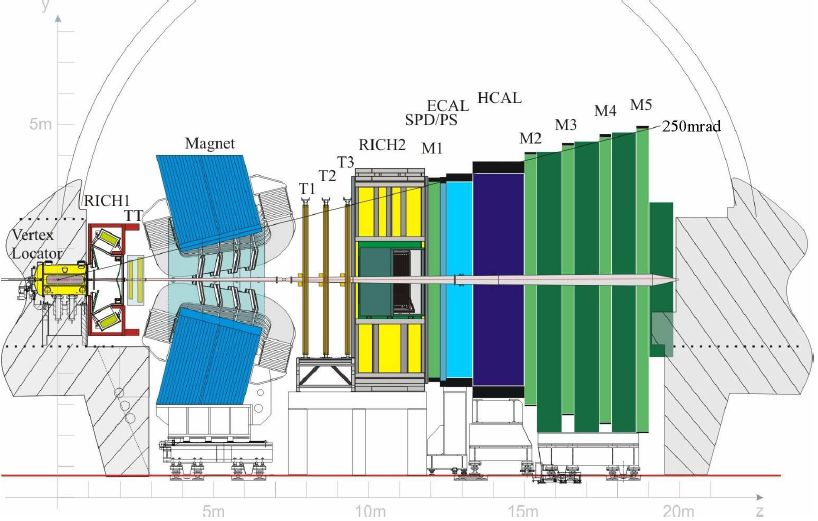
\includegraphics[width=\textwidth]{detektor}
\caption{Schnitt durch die (y,z)-Ebene des LHCb-Detektors. Die Abbildung wurde \cite{detector} entnommen.}
\label{fig:detektor}
\end{figure}


\subsection{Spurdetektoren}
Hauptaufgabe der Spurdektektoren ist die Vertex- und Impulsbestimmung geladener Teilchen. Als Hilfsmittel dient ein Dipolmagnet, dessen Feld die Teilchen abgelenkt. Die Teilchen-Trajektorien werden mit den Stationen Vertex Locator (VELO), TT und T1-T3 gemessen, die im Folgenden detaillierter beschrieben werden. Die Ablenkung des Teilchens von seiner ursprünglichen Trajektorie gibt Aufschluss über den Impuls. Das Magnetfeld ist weitestgehend homogen mit einer dominierenden y-Komponente, sodass die Ablenkung hauptsächlich in der (x,z)-Ebene vonstattengeht. Entlang der z-Achse integriert beträgt die Feldstärke insgesamt $\int B\mathrm{d}l = 4\tesla\meter$. Um ladungsabhängige Detektorasymmetrien zu messen, kann die Orientierung des Magnetfeldes umgekehrt werden. \cite{thesis_linn}

\subsubsection{Vertex Locator (VELO)}
Aufgabe des Vertex Locator (VELO) ist die Detektion des Primärvertex (Protonkollisionspunkt) sowie der Sekundärvertices (Zerfallspunkte instabiler Teilchen). Der VELO befindet sich demnach sehr nah am Kollisionspunkt und besteht insgesamt aus 21 Stationen von Siliziumstreifendetektoren. Um Schäden zu vermeiden, besteht der VELO aus zwei beweglichen Hälften, die erst zusammengeführt werden, sobald der Teilchenstrahl im Experiment stabil ist.

\subsubsection{Trigger Tracker (TT)}
Der Trigger Tracker (TT) besteht aus zwei Stationen, die sich vor dem Magneten befinden und eine Detektionsfläche von etwa $8,4\meter^2$ bieten. Sie sind wie der VELO aus Siliziumstreifen aufgebaut und ermöglichen durch ihre x-u-v-x-Anordnung eine dreidimensionale Spurrekonstruktion, wobei die TT-Stationen so aufgebaut sind, dass die Präzision in der horizontalen Ablenkungsebene (x,z) des Magneten am besten ist. Die Auflösung einer einzelnen Teilchenmessung beträgt etwa $50\micro\meter$.

\subsubsection{Inner Tracker (IT)}
Im Zentrum der drei Stationen T1-T3 nach dem Dipolmagneten ist der sogenannte Inner Tracker platziert. Er ist $120\centi\meter$ breit und $40\centi\meter$ hoch, ebenfalls ein Silikonstreifendetektor und besteht aus vier Lagen, die ähnlich wie die TT Stationen aufgebaut sind. Er deckt eine Fläche von etwa $4\meter^2$ ab und erzielt ebenfalls eine Ortsauflösung von $50\micro\meter$.

\subsubsection{Outer Tracker (OT)}
Der Outer Tracker bildet den äußeren Teil der Stationen T1-T3, der nicht vom IT abgedeckt wird. Er besteht ebenfalls aus 4 Lagen und ist aus Driftröhrchen aufgebaut, die mit einem Gasgemisch aus Argon (70\%), CO$_2$(28,5\%) und O$_2$ (1,5\%) gefüllt sind. Im Innern der Röhrchen verläuft ein mit Gold beschichteter Anodendraht aus Wolfram. Die räumliche Auflösung eines einzelnen Röhrchens liegt bei $200\micro\meter$.

\subsubsection{Klassifizierung von Spuren} \label{kap:spurklassen}
Je nachdem, welche Detektoren an der Rekonstruktion einer Teilchenspur beteiligt sind, teilt man die Spuren in vier unterschiedliche Kategorien ein:
\begin{itemize}
\item \textbf{VELO Spuren} enthalten Treffer ausschließlich im VELO und dienen hauptsächlich der Rekonstruktion des Primärvertex. Außerdem sind sie Ausgangspunkt für die folgenden Spuralgorithmen
\item Haben die Spuren Messungen im VELO und in den TT-Stationen, spricht man von \textbf{Upstream Spuren}. Hierbei handelt es sich dann um Teilchen mit kleinem Impuls, da der Magnet die Teilchen so stark ablenkt, dass jene den Akzeptanzbereich des Detektors verlassen und die anschließenden Detektoren nicht mehr passieren.
\item Bei \textbf{Downstream Spuren} gibt es nur zugeordnete Treffer in den Stationen TT und T1-T3. Diese treten vor allem bei den Zerfallsprodukten langlebiger Teilchen wie dem $\Kshort$ auf, die den VELO vor ihrem Zerfall verlassen. In dieser Arbeit werden ausschließlich Downstream Spuren zur Rekonstruktion der $\Kshort$-Mesonen verwendet (siehe dazu auch Kapitel \ref{kap:downstream})
\item Gibt es zugeordnete Messungen in allen Subdetektoren (VELO, TT, T1-T3), so spricht man von \textbf{Long Spuren}. Da es hier die meisten Messpunkte gibt, haben diese Spuren die präziseste Impuls- und Ortsauflösung. \cite{thesis_linn}
\end{itemize}

\subsection{Detektoren zur Teilchenidentifikation}
Neben der Rekonstruktion der Spuren ist es natürlich essentiell, auch die Teilchensorten zu identifizieren. Hierzu werden die Informationen der Detektoren RICH1/2, SPD, PS HCAL, ECAL sowie M1-M5 verwendet, um eine Teilchenhypothese aufzustellen.

\subsubsection{Die Ring Imaging Cherenkov Detektoren (RICH)}
Die beiden RICH Detektoren nutzen die Cherenkov-Strahlung, um Teilchen voneinander zu unterscheiden, insbesondere $\pi^{\pm}$ und $K^{\pm}$. Ähnlich dem Machschen Kegel bei Schall emittieren geladene Teilchen Photonen in Kegelform, wenn sie ein Medium mit einer Geschwindigkeit $v$ passieren, die größer ist als die Lichtgeschwindigkeit $c'=c/n$ in diesem Medium ($n:$ Brechungsindex des Mediums). Für den Öffnungswinkel $\theta_{\text{C}}$ des Lichtkegels gilt dann:
\begin{align}
\cos \theta_{\text{C}} = \frac{c}{vn}.
\end{align}
Durch Messung des Öffnungswinkels und der Impulsinformation aus den Spurdetektoren lässt sich die Teilchenmasse bestimmen und somit eine Teilchenhypothese aufstellen. RICH1 ist dabei für kleine Impulse im Bereich von $1\giga\electronvolt$ bis $60\giga\electronvolt$ zuständig und deckt den kompletten Akzeptanzbereich des Detektors ab, RICH2 arbeitet dagegen bei Impulsen von $15\giga\electronvolt$ bis $100\giga\electronvolt$ und deckt einen Winkelbereich von ca. $15\milli\rad$ bis $120\milli\rad$ in horizontaler und $100\milli\rad$ in vertikaler Ebene ab.

\subsubsection{Kalorimetersystem}
Das Kalorimetersystem dient zur Identifikation von Elektronen, Photonen sowie Hadronen und soll deren Energie und Position bestimmen. Durch Wechselwirkung mit dem Kalorimetermaterial erzeugen jene einen kaskadenartigen Zerfall. Bei den Subdetektoren des Systems handelt es sich um Szintillationsdetektoren. Diese sind im Einzelnen:
\begin{itemize}
\item Der \textbf{Scintillating Pad Detector (SPD)} kann nur geladene Teilchen detektieren und dient damit der Unterscheidung von Photonen und Elektronen.
\item Auf den SPD und eine $12\milli\meter$ dicke Bleiplatte folgt der \textbf{Preshower Detector (PS)}. Die Platte löst Kaskaden von Photonen und Elektronen aus. Hadronische Kaskaden beginnen erst später und können damit unterschieden werden.
\item Das \textbf{elektromagnetische Kalorimeter (ECAL)} besteht im Wechsel aus Blei- und Szintillatorplatten und detektiert Photonen- und Elektronenschauer.
\item Beim \textbf{hadronischen Kalorimeter (HCAL)} wechseln sich Eisen- und Szintillatorplatten ab. Es ist sensitiv für hadronische Kaskaden.
\end{itemize}

\subsubsection{Myonkammern}
Der LHCb-Detektor besitzt insgesamt 5 Myonenkammern (M1-M5). Zur Verbesserung der Impulsmessung im Trigger ist M1 vor den Kalorimetern angebracht, die restlichen Kammern am Ende des Detektors. Zwischen M2-M5 befinden sich $80\centi\meter$ dicke Eisenplatten zur Absorption hadronischer Teilchen. Ab einem Impuls von etwa $6\giga\electronvolt$ können die Myonen alle 5 Stationen passieren. \cite{thesis_linn}

\subsection{Trigger}
Aufgabe des Triggers ist es, die Ereignisrate von $40\mega\hertz$ auf ein speicherbares Maß von $2-3\kilo\hertz$ zu reduzieren. Hierzu stehen zwei Stufen zur Verfügung:
\begin{enumerate}
    \item Das \textbf{L0-System} bildet die erste Stufe und senkt die Ereignisrate von den ursprünglichen $40\mega\hertz$ auf $1\mega\hertz$. Es besteht aus individuell angefertigten elektronischen Bauteilen, die vollkommen synchron zu den Kollisionsereignissen arbeiten und bildet damit einen reinen Hardware-Trigger. L0 besitzt drei Subsyteme: Mit Hilfe der Kalorimeter wird versucht, die Transversalenergie von Hadronen, Elektronen und Photonen zu bestimmen, die Myonenkammern liefern Informationen über den Transversalimpuls und das \glqq L0 pile-up\grqq-System nutzt VELO-Informationen, um die Zahl der Proton-Proton-Kollisionen abzuschätzen. All diese Informationen laufen in der \glqq L0 Decision Unit\grqq zusammen, die dann anhand vorgegebener Kriterien entscheidet, welche Ereignisse an die nächste Stufe weitergeleitet werden. Im Wesentlichen nutzt man aus, dass B-Mesonen aufgrund ihrer hohen Masse überwiegend Teilchen mit hohem Transversalimpuls und hoher Transversalenergie produzieren.
    \item Die zweite Stufe bildet der softwarebasierte \textbf{High Level Trigger (HLT)}, die abermals in zwei Stufen unterteilt ist: \textbf{HLT1} und \textbf{HLT2}. Der HLT hat Zugriff auf alle Detektorinformationen und könnte damit prinzipiell die komplette Ereignisfilterung vornehmen. Aufgrund der immer noch hohen Ereignisrate von $1\mega\hertz$ am Ausgang des L0-Systems muss darauf jedoch verzichtet und nur ein Teil der Informationen verwendet werden. Die Hauptaufgabe des HLT1 ist die Verifizierung der von L0 getroffenen Entscheidungen. Er ist weiterhin dafür zuständig, entsprechend der Kandidaten aus L0 die Teilchen zu rekonstruieren. Dadurch wird die Ereignisrate auf etwa $30-40\mega\hertz$ gesenkt. Bei dieser Rate ist es nun dem HLT2 möglich, eine vollständige Mustererkennung durchzuführen und somit die Zerfälle des B-Mesons zu rekonstruieren, was in einer Ereignisrate von etwa $2-3\kilo\hertz$ resultiert. 
\end{enumerate}
Bei dieser Ereignisrate ist es nun möglich, die Informationen des Detektors zu speichern und im Anschluss je nach Bedarf die Ereignisfilterung zu verfeinern \cite{detector}.